\section{Design}

% This is where the logical / abstract contribution of the project is presented.

% Notice that, when describing a software project, three dimensions need to be taken into account: structure, behaviour, and interaction.

% Always remember to report \textbf{why} a particular design has been chosen.
% Reporting wrong design choices which has been evalued during the design phase is welcome too.

% Which entities need to by modelled to solve the problem?
% %
% (UML Class diagram)

% How should entities be modularised?
% %
% (UML Component / Package / Deployment Diagrams)

%
%
%
\subsection{Dominio}

Il dominio di PiperChat ruota attorno ai seguenti concetti chiave: gli \emph{Utenti}, le \emph{Amicizie}, i \emph{Server} e \emph{Canali}.

Un utente, dopo essersi registrato ed autenticato al sistema, si trova di fronte a due possibilità: poter interagire privatamente con un altri utenti, oppure partecipare a dei server.

%
%
%
\subsubsection{Interazione tramite Direct}

Al fine di permettere l'interazione mediante i \emph{Direct}, due utenti devono, preventivamente, stringere un legame di \emph{amicizia}.

Successivamente ogni utente ha la possibilità di inviare messaggi privati ai propri amici, oppure partecipare ad una sessione.

%
%
%
\subsubsection{Interazione tramite server}

Un utente può partecipare oppure creare dei \emph{Server}.

Alla creazione di un server, l'utente ne diventa proprietario (o \textit{amministratore}).
%
Questo gli permette di accedere alle varie funzionalità di amministrazione come la modifica delle impostazioni, la rimozione degli altri partecipanti e la creazione di canali.

I \emph{Canali} possono essere:
\begin{itemize}
    \item \textbf{Testuali:} luogo dove gli utenti possono inviare messaggi.

    \item \textbf{Multimediali:} luogo dove gli utenti possono partecipare ad una sessione.
\end{itemize}

%
%
%
\subsubsection{Struttura e relazioni}

Di seguito è riportata la struttura del dominio e le interazioni tra le entità precedentemente descritti.

\begin{figure}[H]
    \centering
    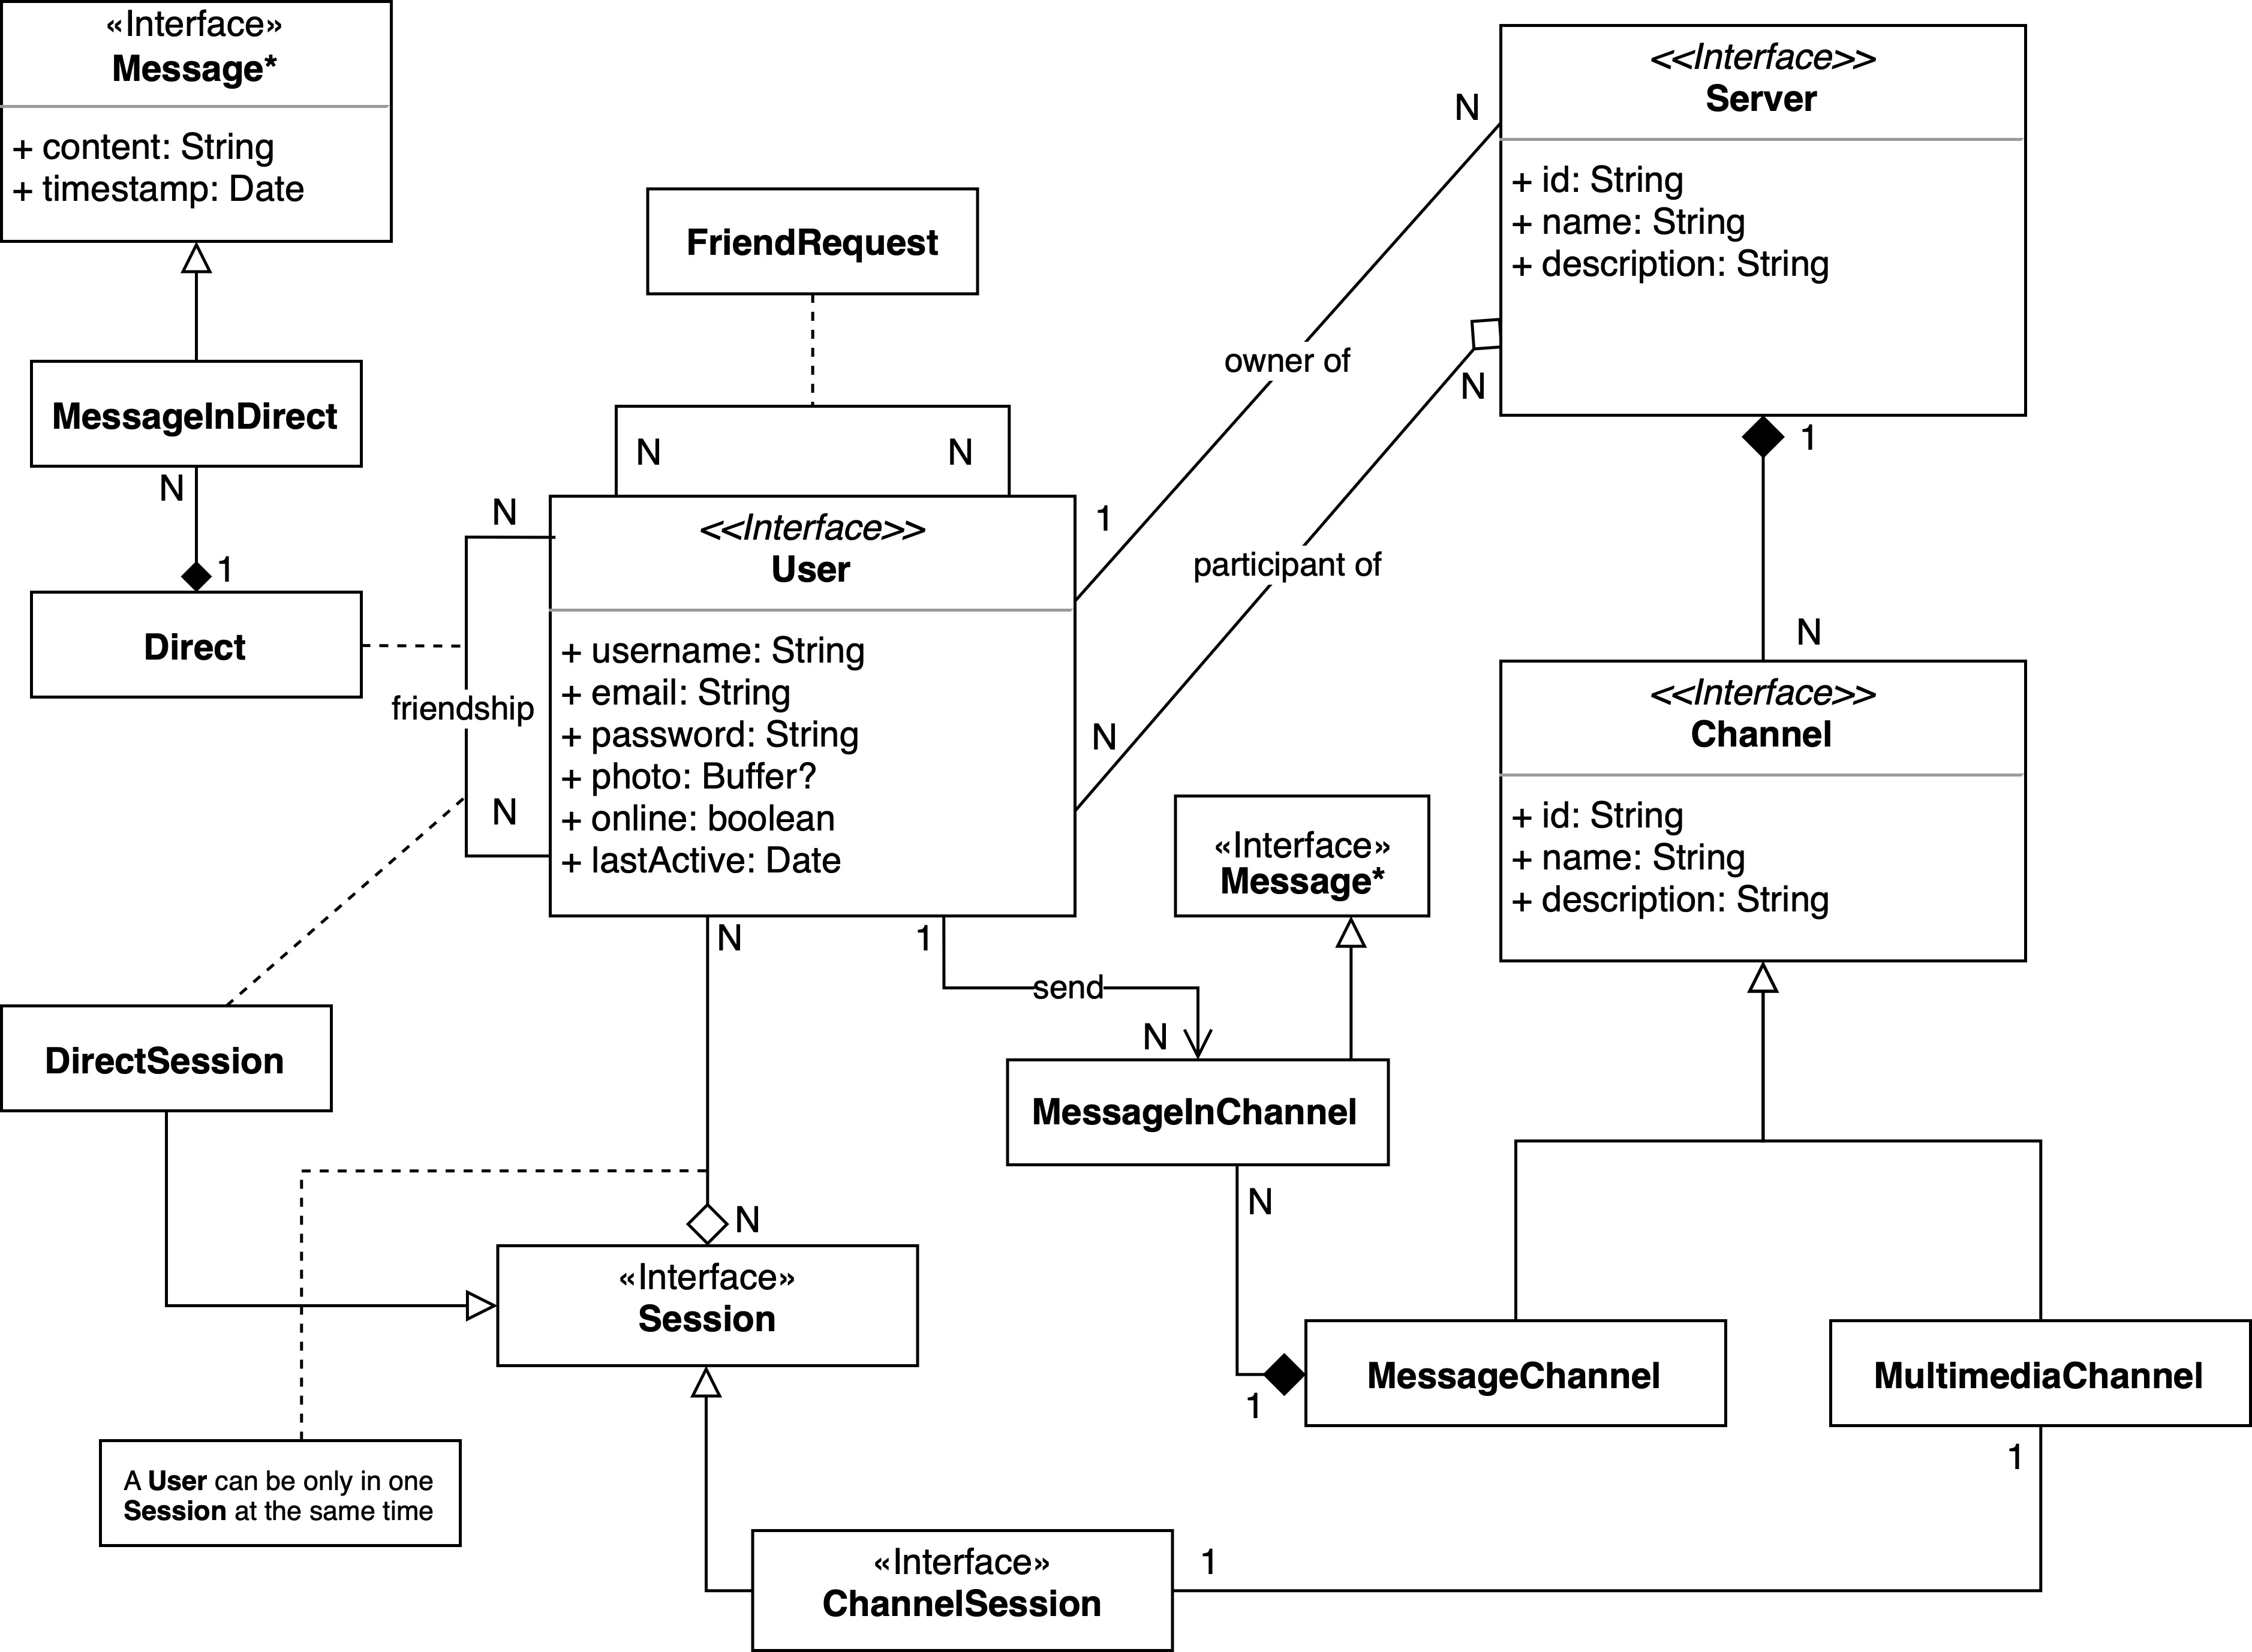
\includegraphics[width=\textwidth]{sections/03-design/img/piperchat-Dominio.jpg}
    \caption{Diagramma delle classi del dominio e le loro relazioni}
    \label{fig:domain}
\end{figure}

%
%
%
\subsection{Microservizi}

Per la realizzzione del sistama si è deciso di adottare un'architettura a \emph{microservizi}, in modo da permette di suddividere la complessità in parti più piccole ad alta coesione, ma accoppiate in modo lasco tra loro.
%
Inoltre, ogni microservizio, se necessario, dispone di un \emph{database}, al quale può accedervi in modo esclusivo.

\begin{figure}[H]
    \centering
    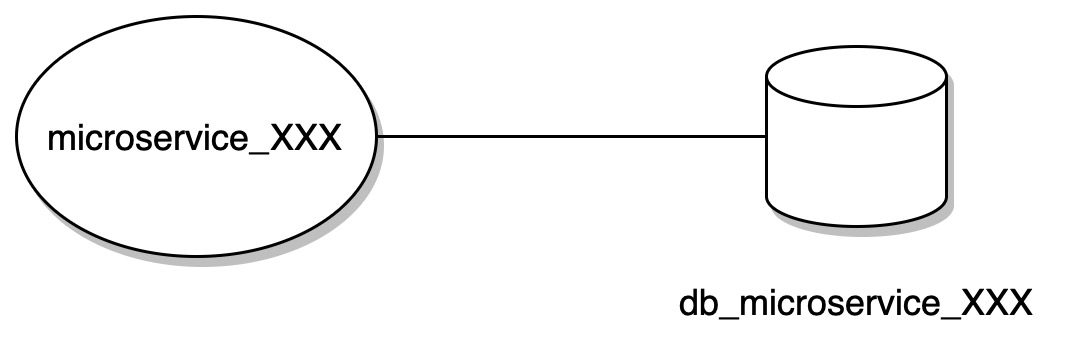
\includegraphics[width=0.82\textwidth]{sections/03-design/img/microservice-db.jpg}
    \caption{Un esempio di microservizio con il proprio database}
    \label{fig:microservice-db}
\end{figure}

A fronte di ciò sono stati identificati i seguenti microservizi:

\begin{itemize}
    \item \textbf{Frontend:} Fornisce l'accesso al sistema servendo la logica del client come \emph{Single Page Application};

    \item \textbf{Messages:} Gestisce i messaggi degli utenti, sia nelle chat individuali, che per i canali testuali;

    \item \textbf{Monitoring:} Permette il monitoraggio degli altri microservizi;

    \item \textbf{Multimedia:} Gestisce tutto ciò che concerne \emph{WebRTC}, permettendo di istanziare sessioni (e quindi chiamate video-audio) all'interno del sistema.
    
    \item \textbf{Notifications:} Permette la gestione delle notifiche e lo status degli utenti del sistema (online, ultimo accesso);

    \item \textbf{Piperchat:} Gestisce la struttura di server e dei canali del sistema;

    \item \textbf{Users:} Gestisce l'autenticazione degli utenti al sistema e tutti i dati relativi agli stessi. Inoltre, si occupa di gestire le amicizie fra utenti;
\end{itemize}

%
%
%
\subsubsection{Moduli}

Per quanto riguarda la gestione dei moduli dell'applicazione si è scelto di optare per lo sviluppo di un modulo indipendente per ogni servizio.

Tuttavia sono presenti i seguenti moduli comuni:

\begin{itemize}
    \item \textbf{Commons}: contiene le funzionalità/utilities comuni a tutti i servizi.

    \item \textbf{Api}: contiene la definizione delle varie API, con le relative interfacce di richieste e risposte in modo da permettere tipizzazione sia lato backend, che lato frontend in cui sappiamo che richieste inviare e che risposte aspettarci.

    \item \textbf{Messages-Api}: contiene la definizione di tutte le tipologie di eventi che vengono inviati al broker dai vari servizi. Rappresenta l'insieme degli eventi interni al sistema.
\end{itemize}

\begin{figure}[H]
    \centering
    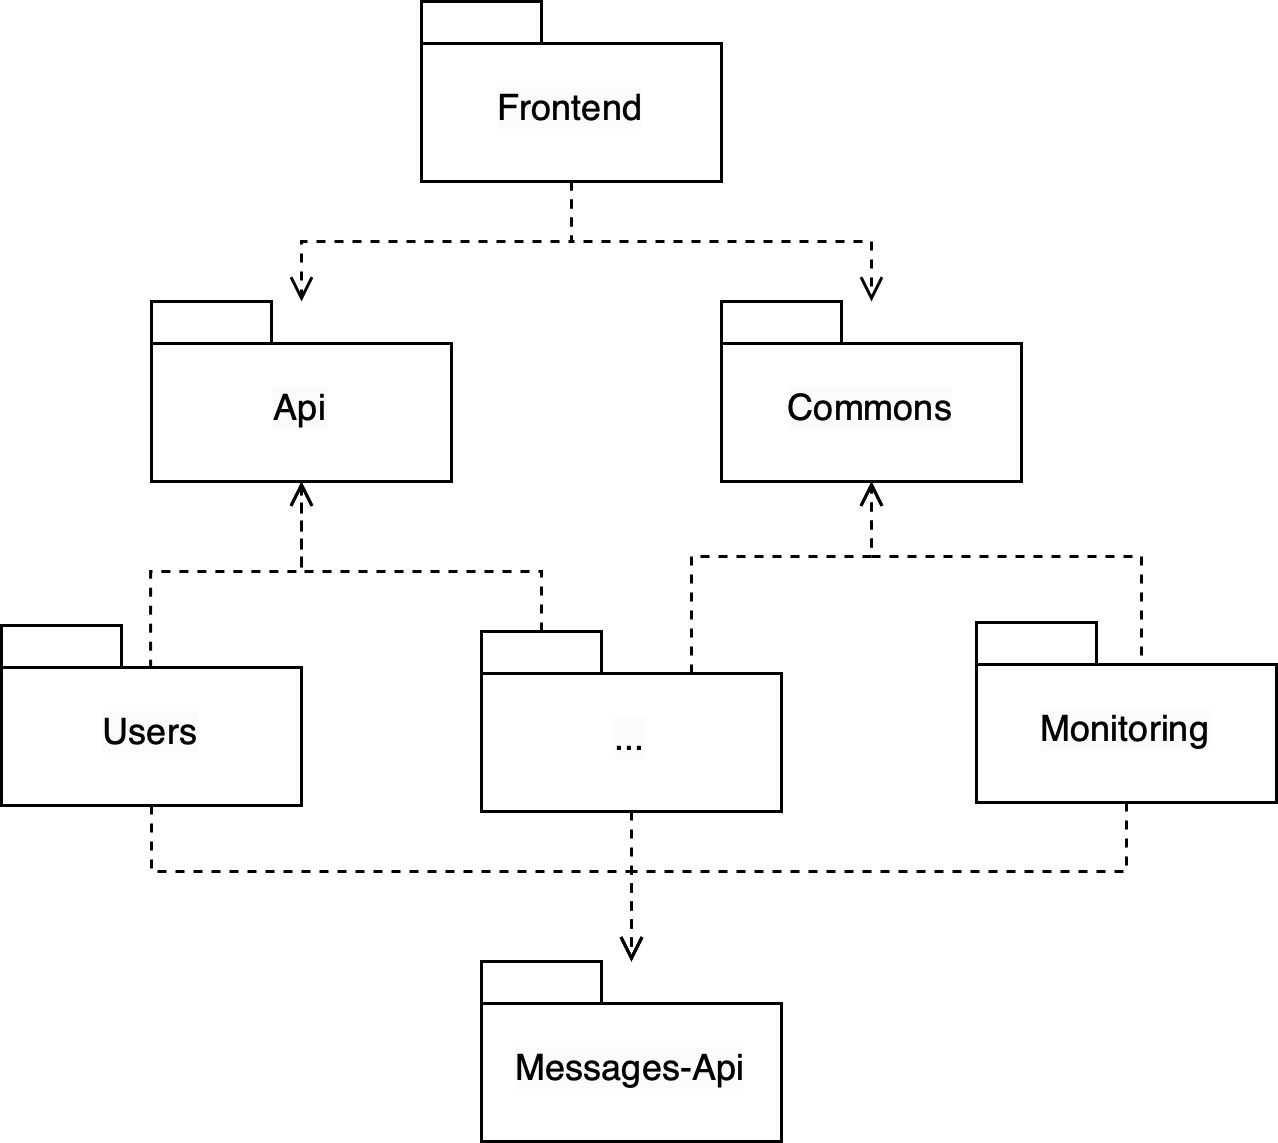
\includegraphics[width=0.8\textwidth]{sections/03-design/img/piperchat-Modules.jpg}
    \caption{Diagrammi dei package Piperchat}
    \label{fig:piperchat-modules}
\end{figure}

%
%
%
\subsection{Comportamento}

% How should each entity behave?
% %
% (UML State diagram or Activity Diagram)

Di seguito, vengono descritti nel dettaglio i comportamenti dei vari microservizi presenti nel sistema.

%
%
%
\subsubsection{Users Service}

Microservizio responsabile della gestione degli utenti e tutte le operazioni relative a quest'ultimi, fra cui:

\begin{itemize}
    \item Creazione degli utenti nel sistema (Registrazione)
    \item Autenticazione degli utenti nel sistema (Login)
    \item Modifiche al profilo dei singoli utenti del sistema
    \item Gestione delle amicizie fra utenti
\end{itemize}

%
%
%
\subsubsection{Piperchat Service}

Microservizio relativo ai server e ai canali, gestisce tutte le operazioni quali:

\begin{itemize}
    \item Operazioni CRUD relative al concetto di Server
    \item Operazioni CRUD relative al concetto di Canali all'interno di Server
\end{itemize}

%
%
%
\subsubsection{Messages Service}

Microservizio relativo alla messaggistica.
%
Si occupa della gestione delle comunicazioni testuali tra gli utenti all'interno della piattaforma PiperChat, sia per chat dirette tra utenti che per i canali testuali.

\begin{itemize}
    \item \textbf{Messaggi Diretti:} il microservizio gestisce l'invio e la ricezione di messaggi diretti tra due utenti. Questa funzionalità è utilizzata per le conversazioni private.
    
    \item \textbf{Canali di Chat:} permette agli utenti di utilizzare le chat all'interno dei canali testuali dei server.

    \item \textbf{Gestione dei Messaggi:} il microservizio gestisce l'archiviazione e il recupero dei messaggi inviati, consentendo agli utenti di accedere alla cronologia dei messaggi in un canale specifico o in una conversazione diretta.
\end{itemize}

%
%
%
\subsubsection{Multimedia Service}

Il microservizio si occupa della gestione delle chiamate multimediali tramite l'utilizzo del concetto di sessione multimediale, sia per le conversazioni dirette tra due utenti, che per i canali.

%
%
%
\subsubsection{Notifications Service}

Il microservizio si occupa di gestire la comunicazione real-time con i client.
Esso si occupa sia di inviare al client tutte le notifiche su eventi che lo riguardano e tiene inoltre traccia degli utenti connessi, andando a rendere disponibili tali informazioni tramite API per ottenere lo stato di un determinato utente.

%
%
%
% \paragraph{Notifiche inviate ai client}

% Le tipologie di notifica che vengono inviate ai client sono le seguenti:

% \begin{itemize}
%     \item \textbf{NewMessageOnChannel}: Relativo solamente ai server di cui l'utente è partecipante.
%     \item \textbf{NewMessageOnDirect}: Relativo soltanto ai direct che coinvolgono l'utente.
%     \item \textbf{FriendRequest}: Relativo alle richieste di amicizia per l'utente.
%     \item \textbf{FriendRequestAccepted}: Relativo alle richieste di amicizia inviate dall'utente.
%     \item \textbf{UserOnline}: Relativo solo agli amici dell'utente o agli utenti che sono partecipanti di uno stesso server dell'utente.
%     \item \textbf{UserOffline}: Relativo solo agli amici dell'utente o agli utenti che sono partecipanti di uno stesso server dell'utente.
%     \item \textbf{ServerUpdated}: Relativo soltanto ai server di cui l'utente è partecipante.
%     \item \textbf{ServerDeleted}: Relativo soltanto ai server di cui l'utente è partecipante.
%     \item \textbf{UserJoinedServer}: Relativo soltanto ai server di cui l'utente è partecipante.
%     \item \textbf{UserLeftServer}: Relativo soltanto ai server di cui l'utente è partecipante.
%     \item \textbf{ChannelCreated}: Relativo soltanto ai server di cui l'utente è partecipante.
%     \item \textbf{ChannelUpdated}: Relativo soltanto ai server di cui l'utente è partecipante.
%     \item \textbf{ChannelDeleted}: Relativo soltanto ai server di cui l'utente è partecipante.
% \end{itemize}

% Lo scopo di tali notifiche è avvisare il client di cosa sia cambiato in modo che possa aggiornarsi senza dover ricaricare tutti i dati tramite meccanismi di polling.
% Questo ha contribuito a rendere l'applicazione reattiva anche lato client.

%
%
%
\subsubsection{Monitoring Service}

Il microservizio si occupa del monitoraggio dello stato operativo dei servizi, eseguendo regolarmente verifiche per stabilire se si trovino in uno stato online o offline.
%
% Questo processo avviene attraverso un meccanismo di polling, in cui il microservizio esegue periodicamente richieste mirate alle route di health check di ciascun servizio.
% %
% Questo approccio permette di ottenere una panoramica accurata e aggiornata della salute complessiva del sistema, garantendo un controllo proattivo e tempestivo sulle condizioni operative dei servizi monitorati.

\subsection{Interazione}

% How should entities interact with each other?
% %
% (UML Sequence Diagram)

Al fine di garantire sia una comunicazione interna fra i microservizi, che una comunicazione verso l'esterno, sono stati identificati e realizzati i seguenti componenti:

\begin{itemize}
    \item \textbf{API Gateway:} componente che permette la comunicazione tra i client esterni al sistema, con i microservizi. Si occupa di redirezionare le richieste agli appositi servizi.

    \item \textbf{Broker:} componente che permette la comunicazione interna al sistema, fra i microservizi stessi.
\end{itemize}

\begin{figure}[htbp]
    \centering
    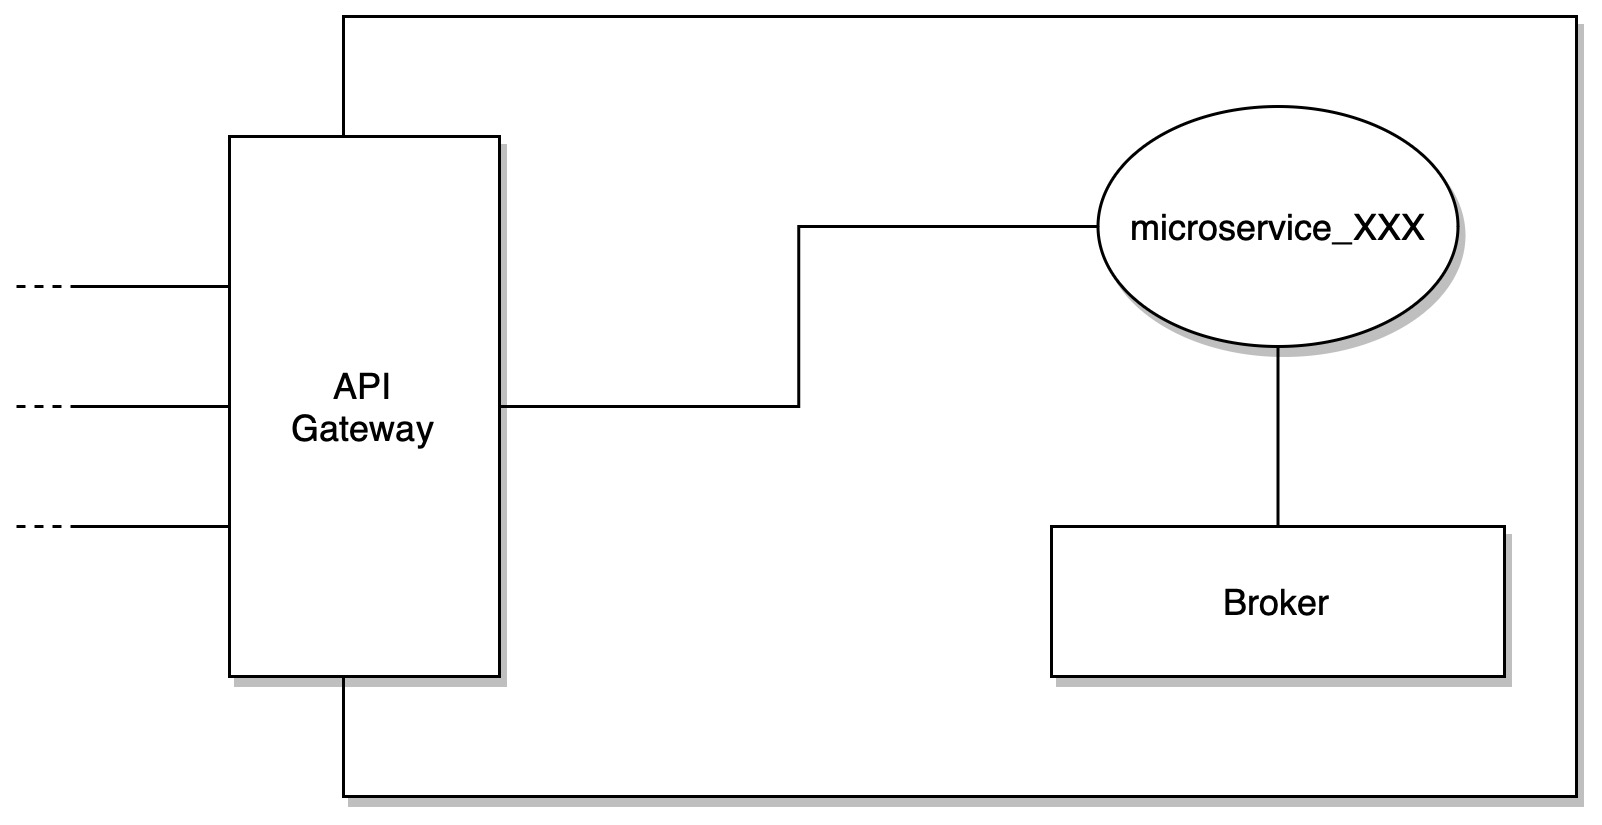
\includegraphics[width=\textwidth]{sections/03-design/img/gateway-broker-microservice.jpg}
    \caption{Un microservizio collegato al Broker e all'API Gateway}
    \label{fig:gateway-broker-microservice}
\end{figure}

%
%
%
\subsubsection{Eventi}
  
Di seguito sono riportate le interazioni che hanno i microservizi tra loro per quanto riguarda gli eventi che ricevono ed inviano:

%
%
%
\paragraph{Servizio Utenti}
Per quanto riguarda il servizio degli utenti, esso non ascolta nessuna tipologia di evento ma produce tutti gli eventi relative alla creazione/modifica degli utenti e delle richieste di amicizia in modo che gli altri servizi possono ricostruire lo stato degli utenti e delle amicizie tra di loro.

\begin{figure}[H]
    \centering
    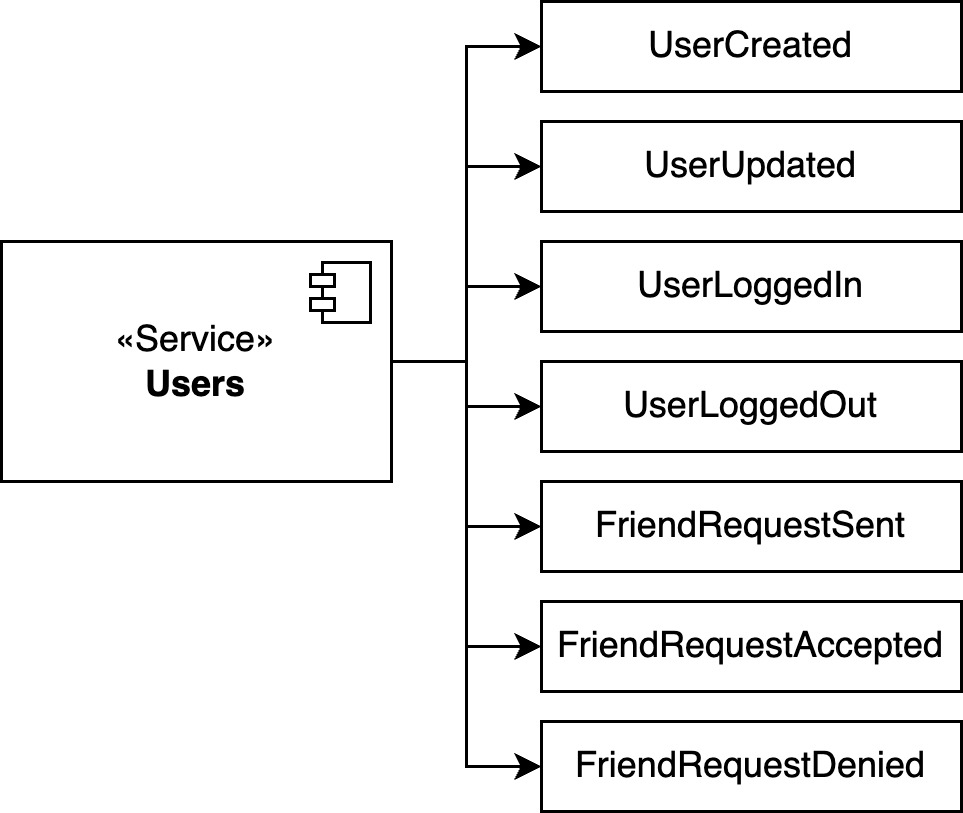
\includegraphics[width=0.55\textwidth]{sections/03-design/img/events/piperchat-EventiUsers.jpg}
    % \caption{Eventi servizio Users}
    \label{fig:users-events}
\end{figure}

%
%
%
\paragraph{Servizio Piperchat}

Per quanto riguarda il servizio Piperchat anch'esso non ascolta nulla e produce tutti gli eventi relativi ai server/canali e alle partecipazioni/abbandoni dei server da parte degli utenti.
%
In questo modo gli altri servizi possono rimanere sincronizzati su tali informazioni.

\begin{figure}[H]
    \centering
    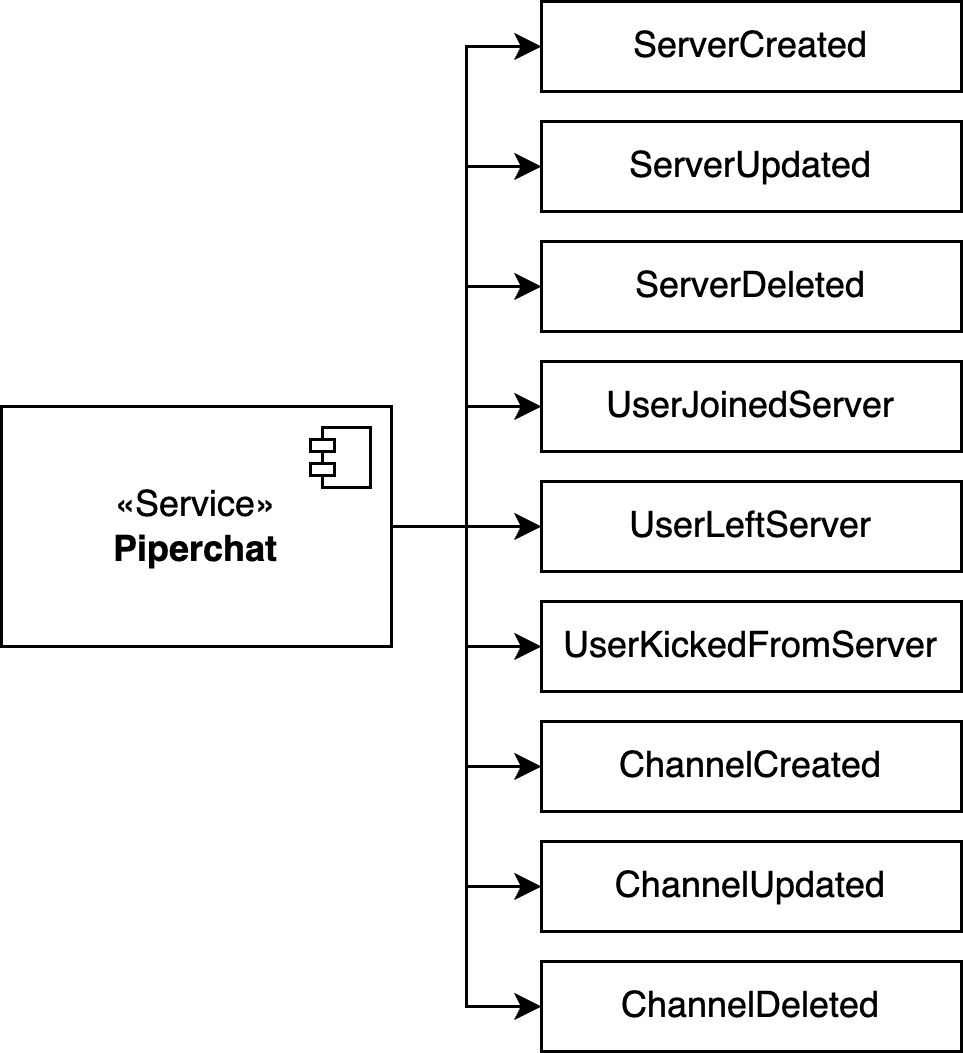
\includegraphics[width=0.55\textwidth]{sections/03-design/img/events/piperchat-EventiPiperchat.jpg}
    % \caption{Eventi servizio Piperchat}
    \label{fig:piperchat-events}
\end{figure}

%
%
%
\paragraph{Servizio Messaggi}

Il servizio messaggi rimane in ascolto per tutti gli eventi che riguardano i canali e le amicizie in modo da sapere se l'invio di un messaggio è possibile.
Inoltre si occupa della produzione degli eventi riguardanti l'invio di nuovi messaggi.

\begin{figure}[H]
    \centering
    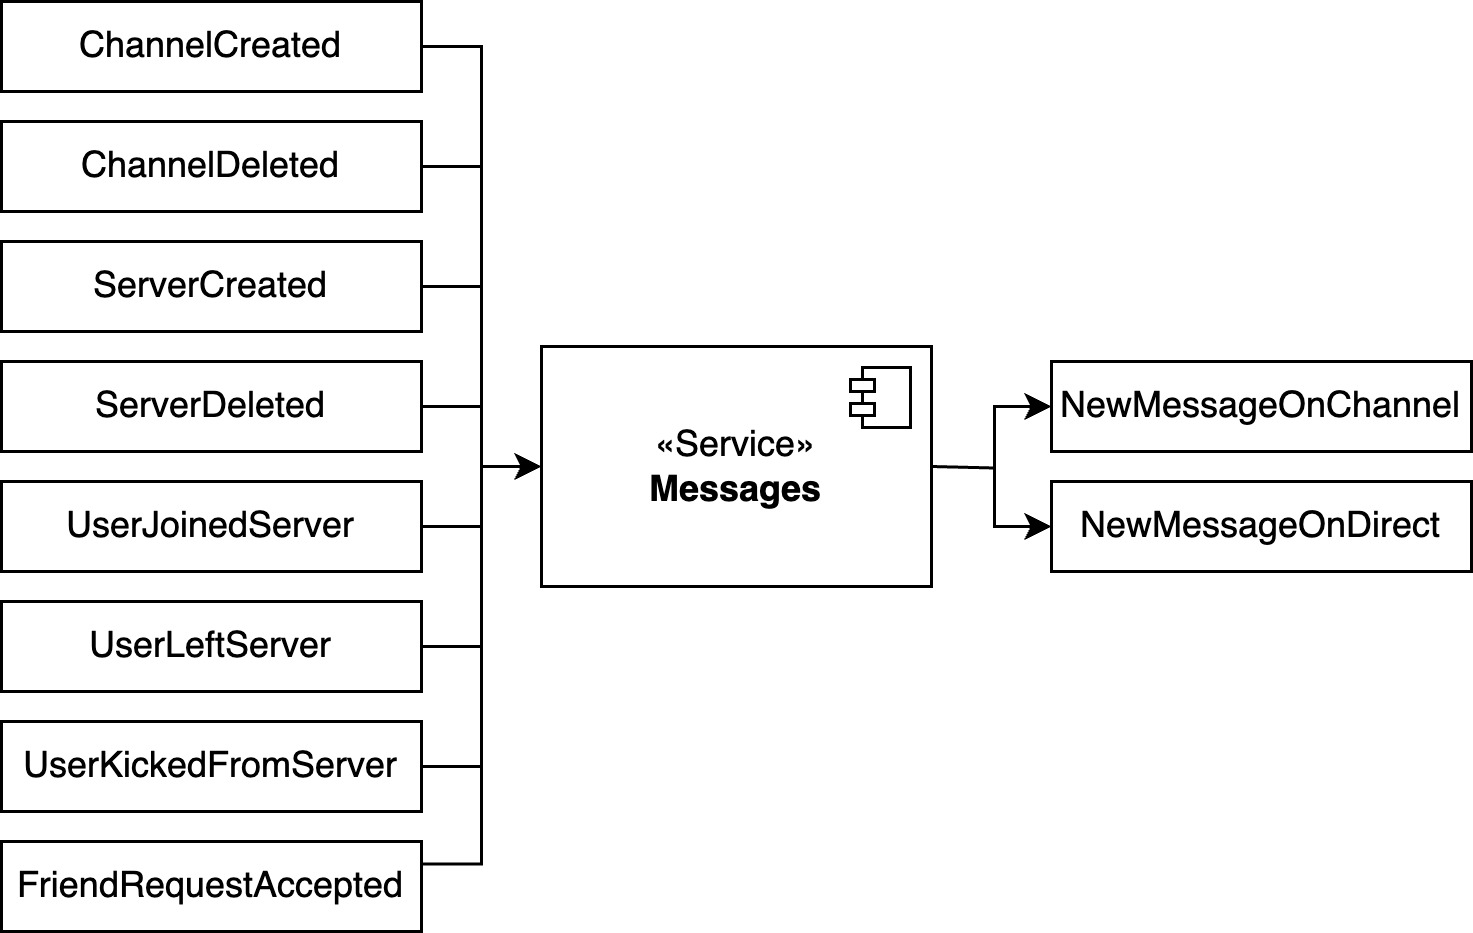
\includegraphics[width=0.9\textwidth]{sections/03-design/img/events/piperchat-EventiMessages.jpg}
    % \caption{Eventi servizio Messages}
    \label{fig:messages-events}
\end{figure}

%
%
%
\paragraph{Servizio Multimedia}

Il servizio che si occupa della gestione delle sessioni multimediali rimane in ascolto degli eventi riguardanti i server e le amicizie anch'esso per capire quando una sessione multimediale tra due utenti o in un server possa essere effettuata.
Si occupa anche della pubblicazione degli eventi riguardanti i join/left delle sessioni da parte degli utenti.

\begin{figure}[H]
    \centering
    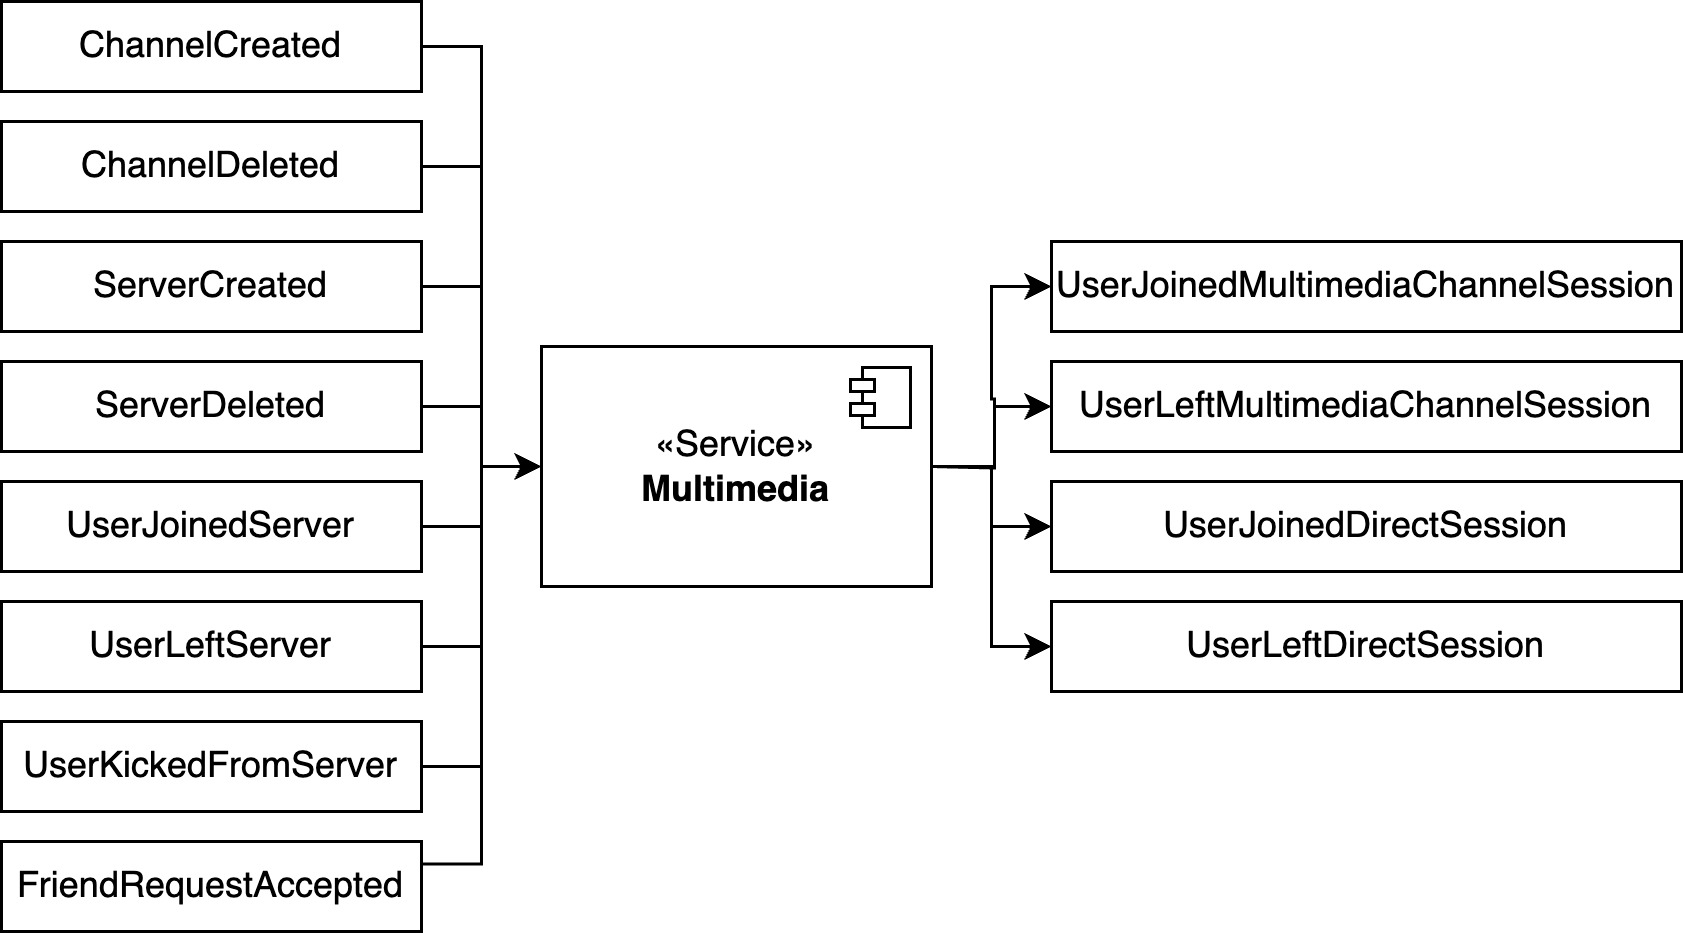
\includegraphics[width=0.9\textwidth]{sections/03-design/img/events/piperchat-EventiMultimedia.jpg}
    % \caption{Eventi servizio Multimedia}
    \label{fig:multimedia-events}
\end{figure}

%
%
%
\paragraph{Servizio Notifiche}

Il servizio di notifiche ascolta la maggior parte degli eventi che propaga agli utenti interessati in modo da rendere l'interfaccia e l'interazione con il servizio reattivi.
Tiene inoltre traccia degli utenti che sono a lui connessi per stabilire il loro status (online/offline/ultimo accesso).

\begin{figure}[H]
    \centering
    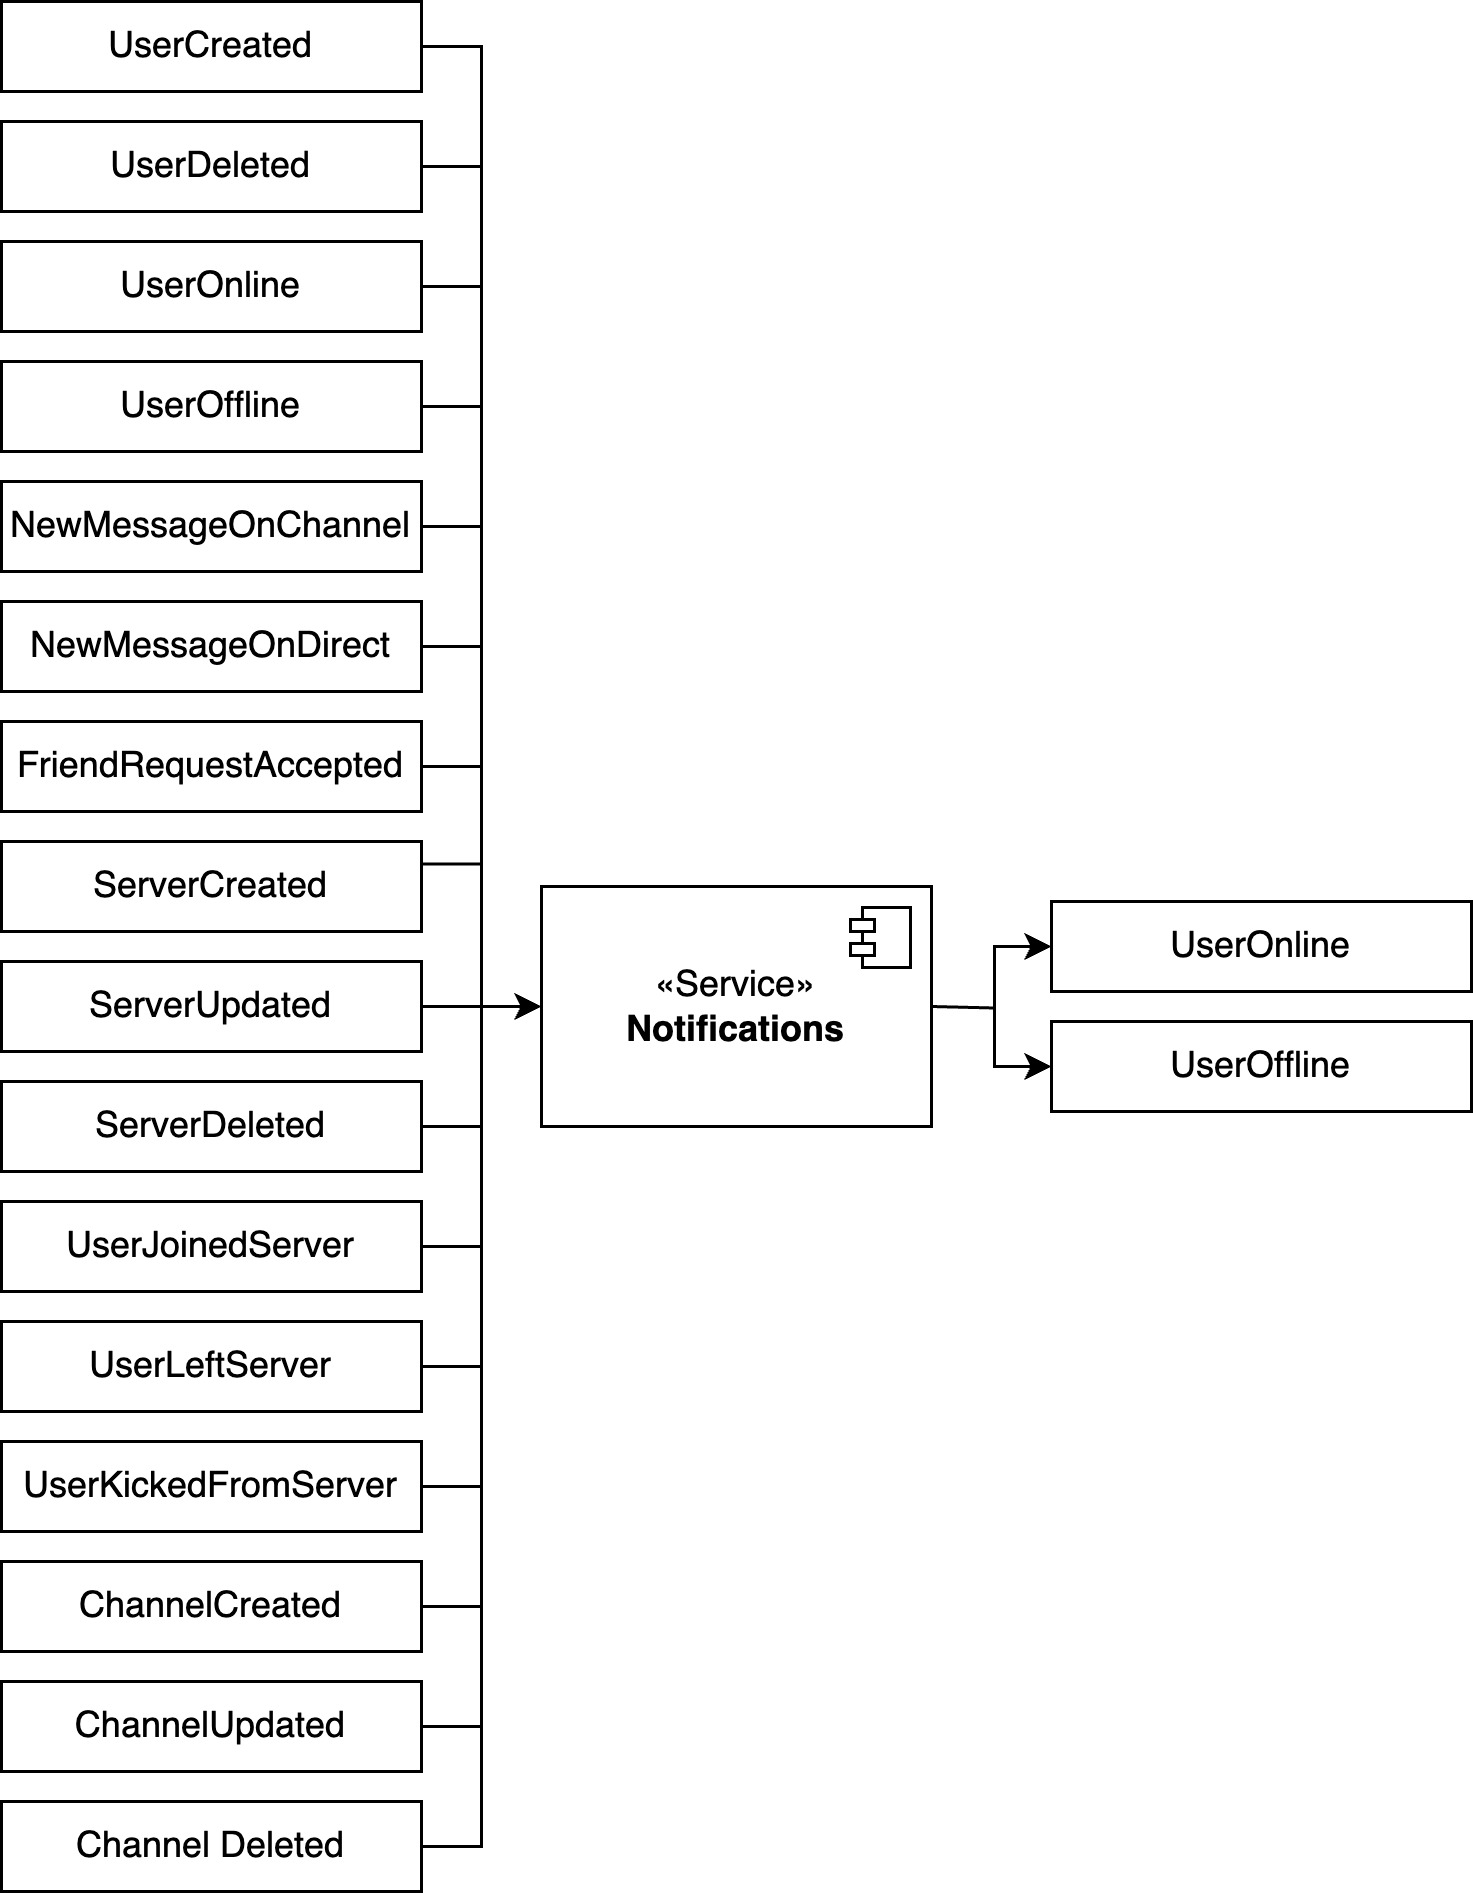
\includegraphics[width=\textwidth]{sections/03-design/img/events/piperchat-EventiNotifications.jpg}
    % \caption{Eventi servizio Notifications}
    \label{fig:notfications-events}
\end{figure}

%
%
%
\subsection{Recap dell'architettura proposta}

Un utente, per accedere al servizio sfrutta l'\emph{API Gateway}.
In questo modo è possibile nascondere l'implementazione retrostante.

Di seguito è riportato lo schema architetturale del sistema.

\begin{figure}[H]
    \centering
    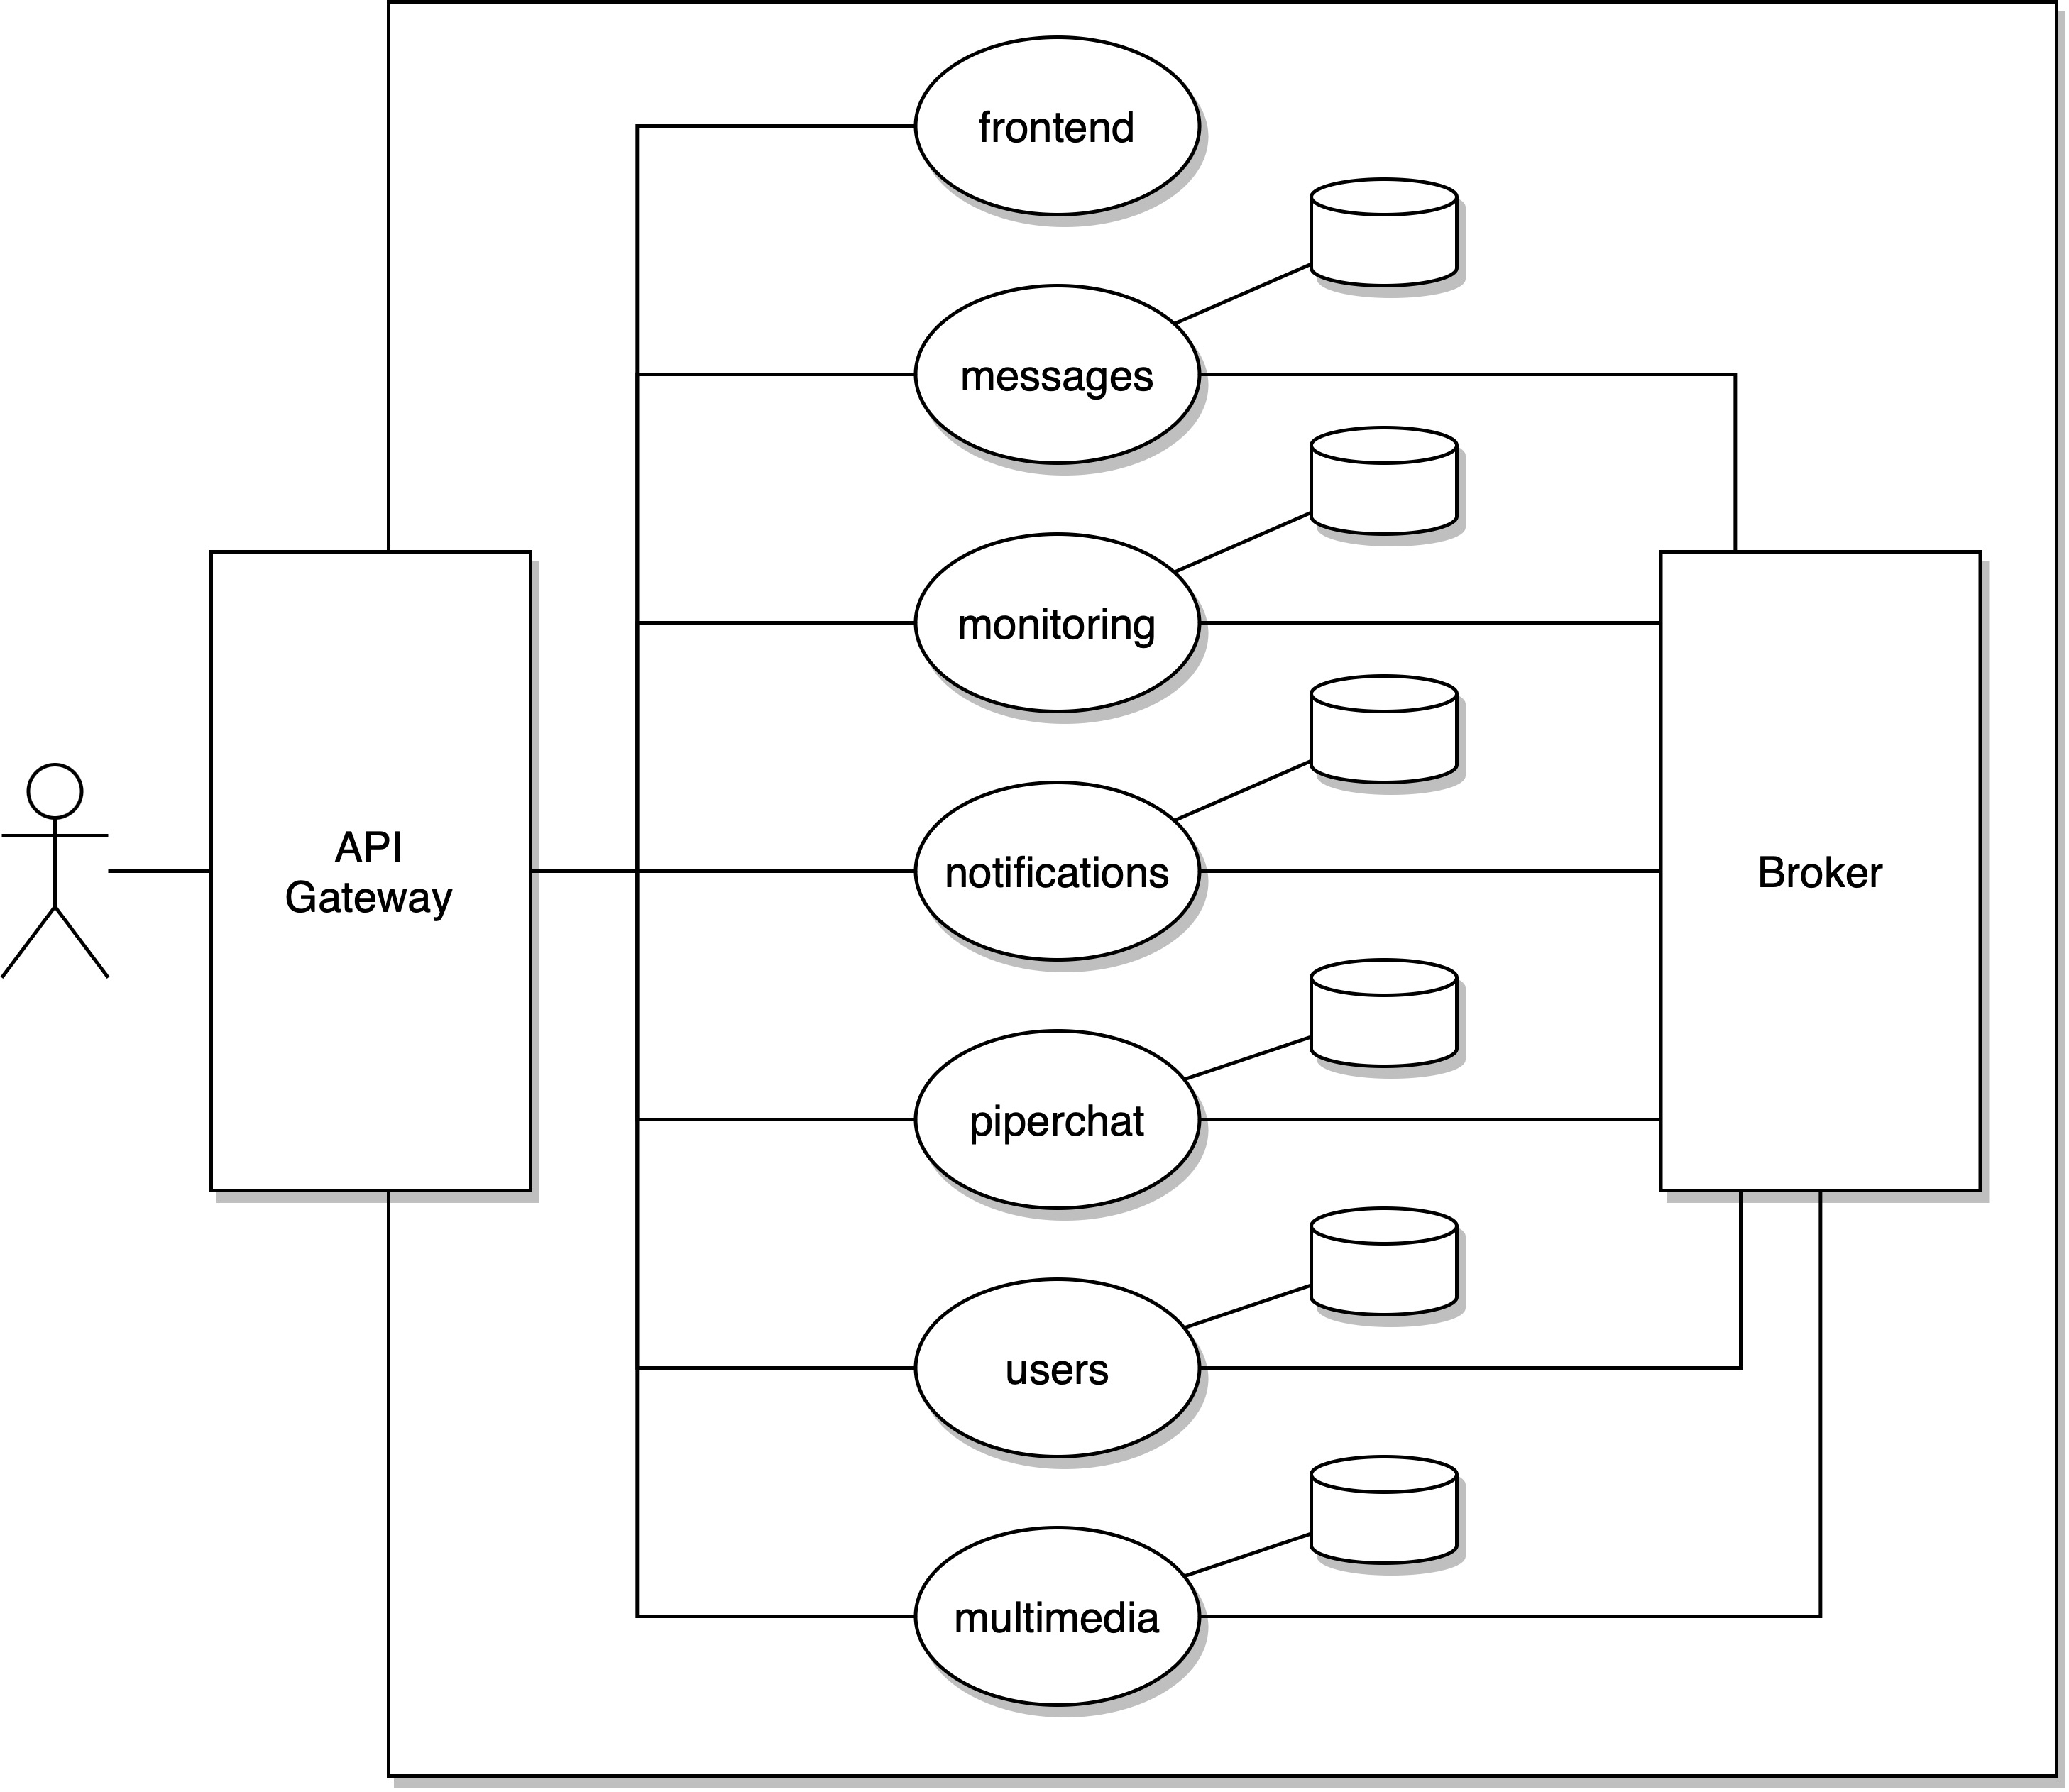
\includegraphics[width=\textwidth]{sections/03-design/img/piperchat-microservizi.jpg}
  %  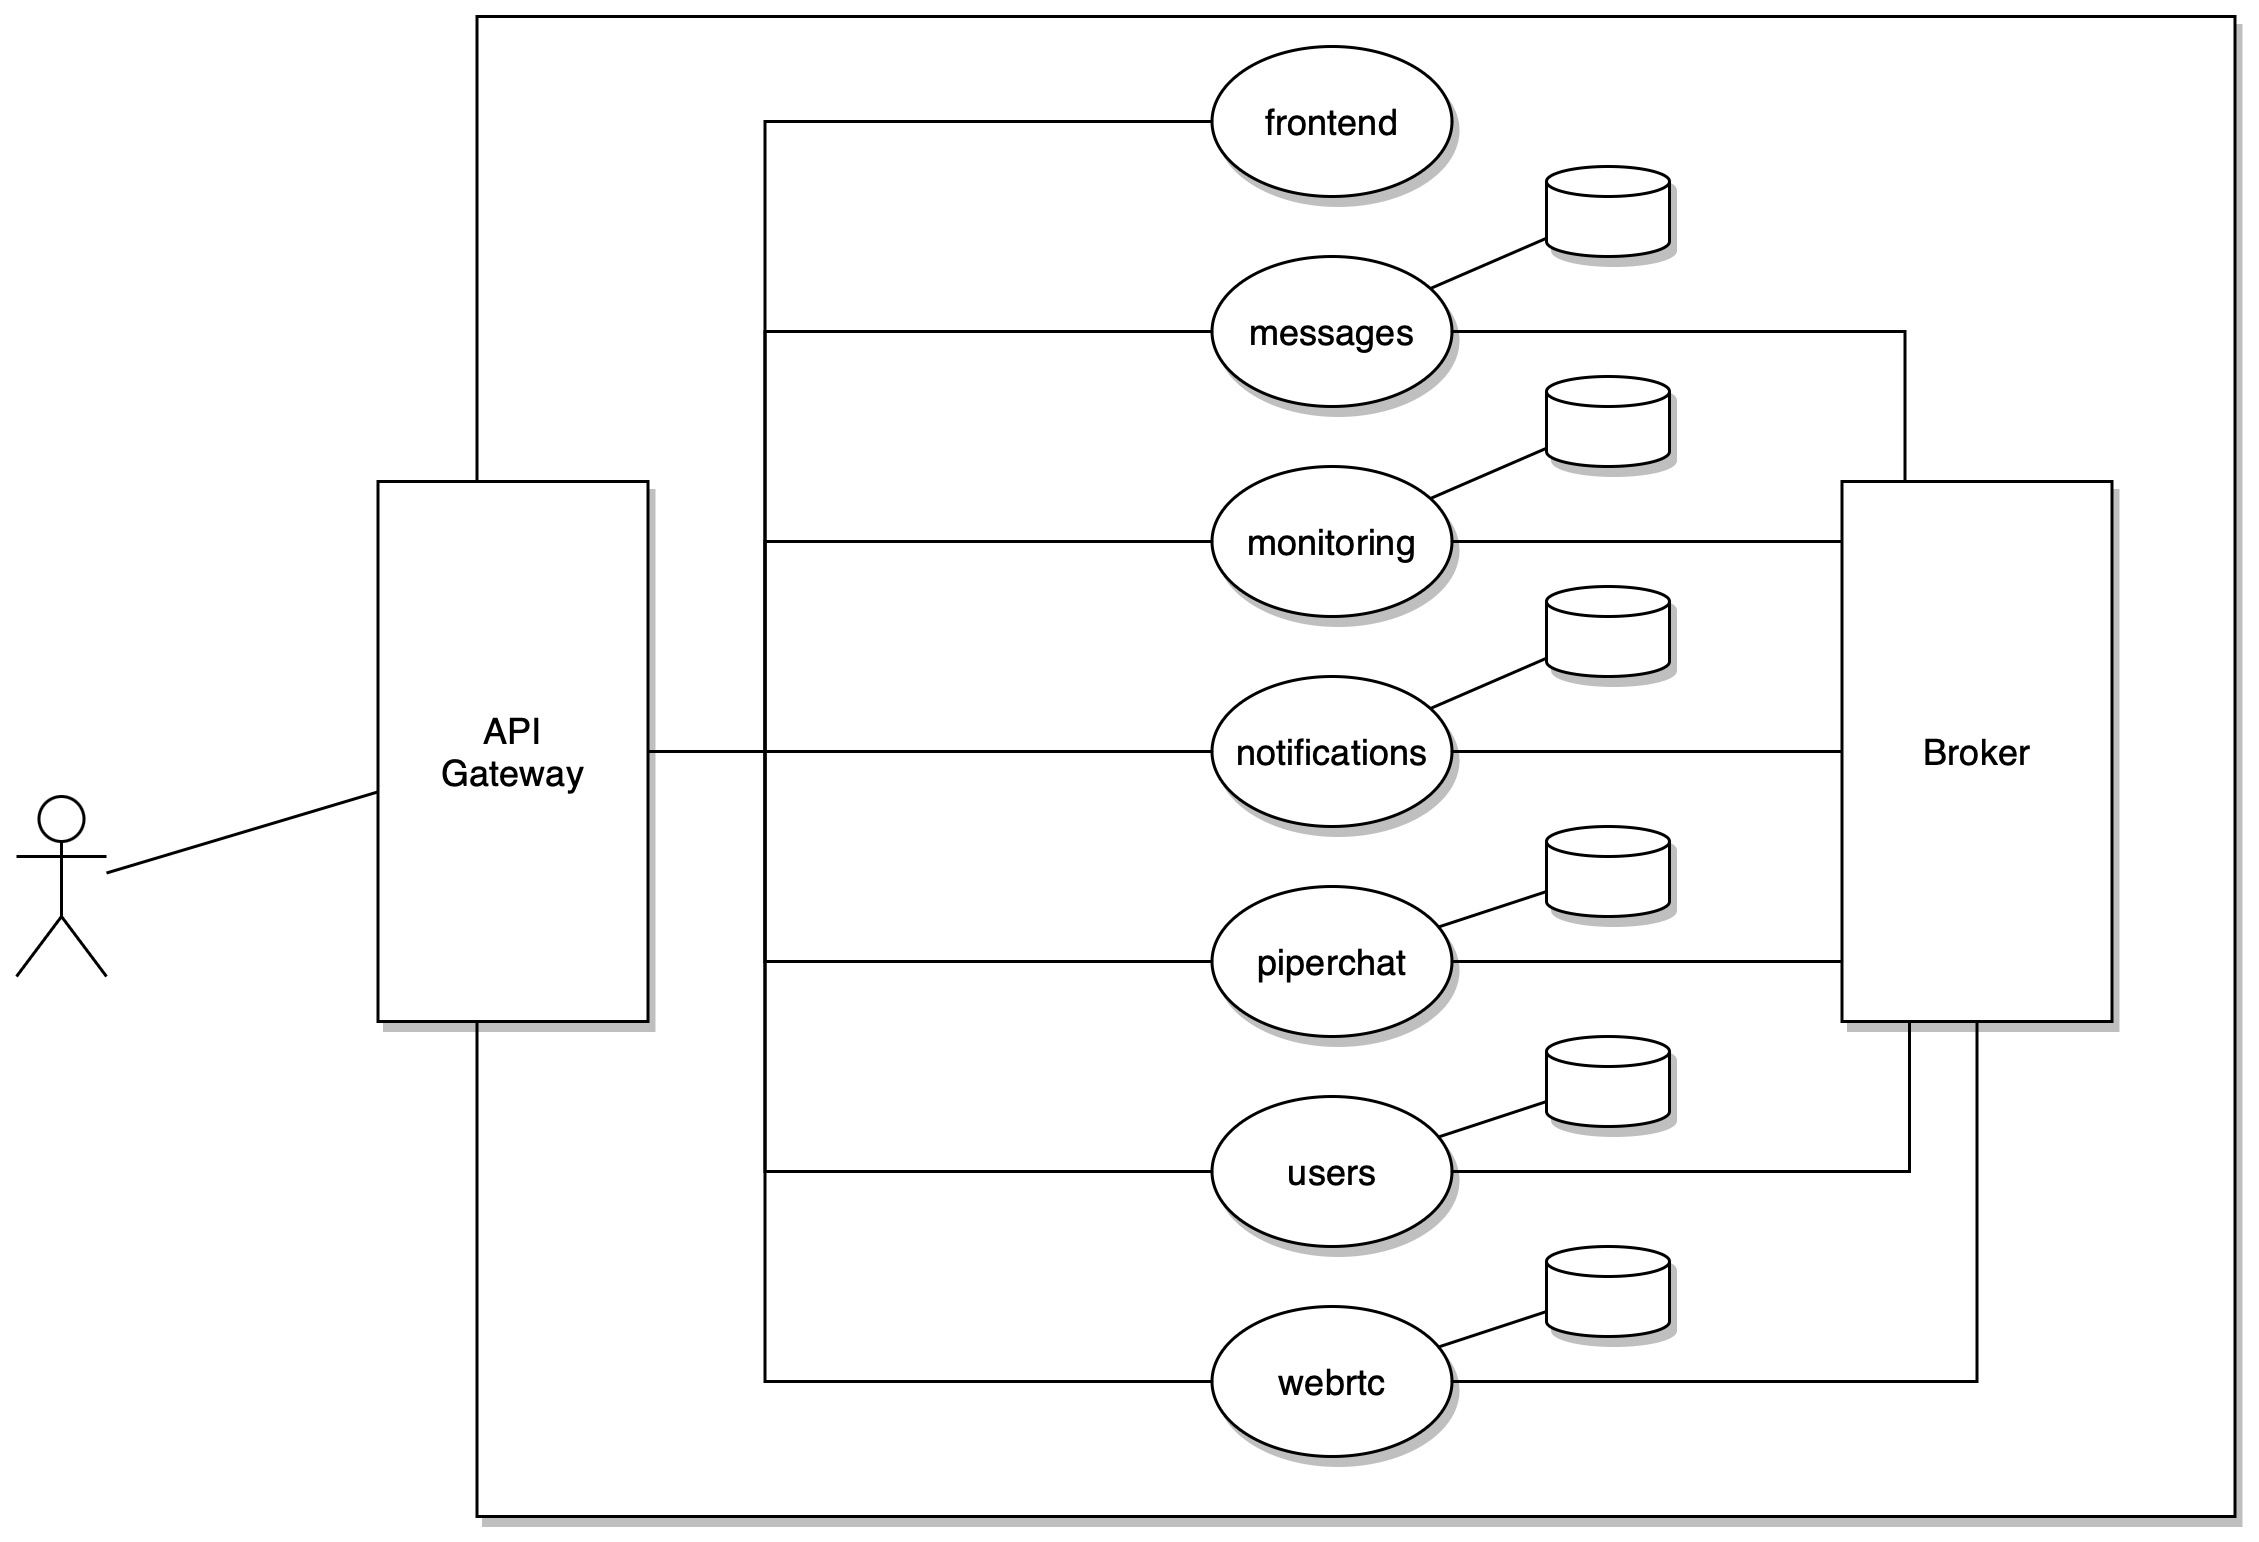
\includegraphics[angle=-90,width=0.95\textwidth]{sections/03-design/img/architecture-schema.jpg}
    \caption{Architettura di Piperchat}
    \label{fig:piperchat-architecture}
\end{figure}
